\chapter{Експериментальна оцінка ентропії на символ джерела
відкритого тексту}

\section{Мета роботи}
Засвоєння понять ентропії на символ джерела та його надлишковості, вивчення та
порівняння різних моделей джерела відкритого тексту для наближеного визначення
ентропії, набуття практичних навичок щодо оцінки ентропії на символ джерела.

\section{Завдання}
0. Уважно прочитати методичні вказівки до виконання комп’ютерного практикуму.

1. Написати програми для підрахунку частот букв і частот біграм в тексті, а також
підрахунку H 1 та H 2 за безпосереднім означенням. Підрахувати частоти букв та біграм, атакож значення H 1 та H 2 на довільно обраному тексті російською мовою достатньої
довжини (щонайменше 1Мб), де імовірності замінити відповідними частотами. Також
одержати значення H 1 та H 2 на тому ж тексті, в якому вилучено всі пробіли.

2. За допомогою програми CoolPinkProgram оцінити значення H ( 10 ) , H ( 20 ) , H ( 30 ) .

3. Використовуючи отримані значення ентропії, оцінити надлишковість російської
мови в різних моделях джерела.

\section{Хід роботи}

%\subsection{Лістинг програми}

\begin{table}[]
\centering
\caption{Ентропія, надлишковість}
\label{tab:my-table}
\begin{tabular}{ll}
\hline
\multicolumn{1}{|l|}{H1 (no spaces)}              & \multicolumn{1}{l|}{4.492315117172669}   \\ \hline
\multicolumn{1}{|l|}{H1 redundancy (no spaces)}   & \multicolumn{1}{l|}{0.10153697656546612} \\ \hline
\multicolumn{1}{|l|}{H2 (no spaces)}              & \multicolumn{1}{l|}{4.1802847959379115}  \\ \hline
\multicolumn{1}{|l|}{H2 redundancy (no spaces)}   & \multicolumn{1}{l|}{0.16394304081241773} \\ \hline
\multicolumn{1}{|l|}{H1 (with spaces)}            & \multicolumn{1}{l|}{4.406442333151592}   \\ \hline
\multicolumn{1}{|l|}{H1 redundancy (with spaces)} & \multicolumn{1}{l|}{0.11871153336968165} \\ \hline
\multicolumn{1}{|l|}{H2 (with spaces)}            & \multicolumn{1}{l|}{2.9080400719491637}  \\ \hline
\multicolumn{1}{|l|}{H2 redundancy (with spaces)} & \multicolumn{1}{l|}{0.4183919856101672}  \\ \hline
\multicolumn{1}{|l|}{H10}                         & \multicolumn{1}{l|}{3.1173 < R < 3.6639}  \\ \hline
\multicolumn{1}{|l|}{H20}                         & \multicolumn{1}{l|}{2.375 < R < 2.7555}  \\ \hline
\multicolumn{1}{|l|}{H30}                         & \multicolumn{1}{l|}{2.56079 < R < 3.0895}  \\ \hline
\end{tabular}
\end{table}


\subsection{Аналіз частот символів}

\begin{table}[]
\centering
\caption{H1 (no spaces)}
\label{tab:my-table}

\begin{tabular}{|l|l|}
\hline
\multicolumn{1}{|c|}{\textbf{о}} & \multicolumn{1}{c|}{\textbf{0.10584822334367971}} \\ \hline
е                                & 0.08399778970225735                               \\ \hline
а                                & 0.0824350401264014                                \\ \hline
н                                & 0.06483252245912892                               \\ \hline
и                                & 0.062443069723669614                              \\ \hline
т                                & 0.06075944449001265                               \\ \hline
л                                & 0.052529107290097264                              \\ \hline
р                                & 0.04690191372068225                               \\ \hline
с                                & 0.04619608621887991                               \\ \hline
в                                & 0.04187478145249371                               \\ \hline
к                                & 0.0377779600505951                                \\ \hline
д                                & 0.03151616927772478                               \\ \hline
у                                & 0.03098086279317743                               \\ \hline
м                                & 0.029899457354636227                              \\ \hline
п                                & 0.027291996736357238                              \\ \hline
я                                & 0.02227997392539382                               \\ \hline
ь                                & 0.022161256761482107                              \\ \hline
ы                                & 0.019676830294893435                              \\ \hline
г                                & 0.019454505424295145                              \\ \hline
з                                & 0.017880963378992674                              \\ \hline
б                                & 0.01760683465505109                               \\ \hline
ч                                & 0.015431072814632862                              \\ \hline
й                                & 0.011353677857737984                              \\ \hline
ж                                & 0.010216151578074883                              \\ \hline
ш                                & 0.009704588526309881                              \\ \hline
х                                & 0.008452662070513678                              \\ \hline
ю                                & 0.0071014448958095                                \\ \hline
щ                                & 0.00427813488860013                               \\ \hline
э                                & 0.004193953626917282                              \\ \hline
ц                                & 0.0033564579978674083                             \\ \hline
ф                                & 0.0013792775952651277                             \\ \hline
ъ                                & 0.00018778896836943055                            \\ \hline
\end{tabular}
\end{table}


% Please add the following required packages to your document preamble:
% Note: It may be necessary to compile the document several times to get a multi-page table to line up properly

\begin{table}[]
\centering
\caption{H2 (no spaces)}
\label{tab:my-table}
\begin{tabular}{ll}
\hline
\multicolumn{1}{|c|}{\textbf{то}} & \multicolumn{1}{c|}{\textbf{0.014304339004416279}} \\ \hline
\multicolumn{1}{|l|}{на}          & \multicolumn{1}{l|}{0.012314207638478175}          \\ \hline
\multicolumn{1}{|l|}{не}          & \multicolumn{1}{l|}{0.011584636703893491}          \\ \hline
\multicolumn{1}{|l|}{ст}          & \multicolumn{1}{l|}{0.010900394140984187}          \\ \hline
\multicolumn{1}{|l|}{по}          & \multicolumn{1}{l|}{0.010889601671537668}          \\ \hline
\multicolumn{1}{|l|}{ал}          & \multicolumn{1}{l|}{0.010874492214312541}          \\ \hline
\multicolumn{1}{|l|}{но}          & \multicolumn{1}{l|}{0.01060683897203887}           \\ \hline
\multicolumn{1}{|l|}{ко}          & \multicolumn{1}{l|}{0.010501072771462984}          \\ \hline
\multicolumn{1}{|l|}{ра}          & \multicolumn{1}{l|}{0.010036996585262668}          \\ \hline
\multicolumn{1}{|l|}{ен}          & \multicolumn{1}{l|}{0.009972241768583552}          \\ \hline
\multicolumn{1}{|l|}{он}          & \multicolumn{1}{l|}{0.009408874863475261}          \\ \hline
\multicolumn{1}{|l|}{ов}          & \multicolumn{1}{l|}{0.009331169083460324}          \\ \hline
\multicolumn{1}{|l|}{ер}          & \multicolumn{1}{l|}{0.00923187836455235}           \\ \hline
\multicolumn{1}{|l|}{от}          & \multicolumn{1}{l|}{0.008839032476699059}          \\ \hline
\multicolumn{1}{|l|}{ка}          & \multicolumn{1}{l|}{0.008672828447222666}          \\ \hline
\multicolumn{1}{|l|}{ро}          & \multicolumn{1}{l|}{0.008627500075547287}          \\ \hline
\multicolumn{1}{|l|}{ос}          & \multicolumn{1}{l|}{0.008349054363827097}          \\ \hline
\multicolumn{1}{|l|}{го}          & \multicolumn{1}{l|}{0.00828861653492659}           \\ \hline
\multicolumn{1}{|l|}{ол}          & \multicolumn{1}{l|}{0.008228178706026084}          \\ \hline
\multicolumn{1}{|l|}{ни}          & \multicolumn{1}{l|}{0.008143997444343236}          \\ \hline
\multicolumn{1}{|l|}{ак}          & \multicolumn{1}{l|}{0.007850442275397919}          \\ \hline
\multicolumn{1}{|l|}{ла}          & \multicolumn{1}{l|}{0.007833174324283487}          \\ \hline
\multicolumn{1}{|l|}{ло}          & \multicolumn{1}{l|}{0.007546094637006083}          \\ \hline
\multicolumn{1}{|l|}{во}          & \multicolumn{1}{l|}{0.007457596387544627}          \\ \hline
\multicolumn{1}{|l|}{пр}          & \multicolumn{1}{l|}{0.007306501815293361}          \\ \hline
\multicolumn{1}{|l|}{ор}          & \multicolumn{1}{l|}{0.007228796035278424}          \\ \hline
\multicolumn{1}{|l|}{ре}          & \multicolumn{1}{l|}{0.007058275018023424}          \\ \hline
\multicolumn{1}{|l|}{ет}          & \multicolumn{1}{l|}{0.00699352020134431}           \\ \hline
\multicolumn{1}{|l|}{ве}          & \multicolumn{1}{l|}{0.006790621775749753}          \\ \hline
\multicolumn{1}{|l|}{ел}          & \multicolumn{1}{l|}{0.006699965032398994}          \\ \hline
\multicolumn{1}{|l|}{ли}          & \multicolumn{1}{l|}{0.00656182142348355}           \\ \hline
\multicolumn{1}{|l|}{од}          & \multicolumn{1}{l|}{0.00649922510069374}           \\ \hline
\end{tabular}
\end{table}


\begin{table}[]
\centering
\caption{H1 (with spaces)}
\label{tab:my-table}
\begin{tabular}{ll}
\hline
\multicolumn{1}{|l|}{}  & \multicolumn{1}{l|}{0.16067119346633524}    \\ \hline
\multicolumn{1}{|c|}{о} & \multicolumn{1}{l|}{0.0888414629727595}     \\ \hline
\multicolumn{1}{|l|}{е} & \multicolumn{1}{l|}{0.07050176458226141}    \\ \hline
\multicolumn{1}{|l|}{а} & \multicolumn{1}{l|}{0.06919010384584726}    \\ \hline
\multicolumn{1}{|l|}{н} & \multicolumn{1}{l|}{0.05441580370018769}    \\ \hline
\multicolumn{1}{|l|}{и} & \multicolumn{1}{l|}{0.05241026718746603}    \\ \hline
\multicolumn{1}{|l|}{т} & \multicolumn{1}{l|}{0.05099715202945077}    \\ \hline
\multicolumn{1}{|l|}{л} & \multicolumn{1}{l|}{0.04408919293007616}    \\ \hline
\multicolumn{1}{|l|}{р} & \multicolumn{1}{l|}{0.039366127267325156}   \\ \hline
\multicolumn{1}{|l|}{с} & \multicolumn{1}{l|}{0.03877370591261876}    \\ \hline
\multicolumn{1}{|l|}{в} & \multicolumn{1}{l|}{0.03514671034037958}    \\ \hline
\multicolumn{1}{|l|}{к} & \multicolumn{1}{l|}{0.03170813012254245}    \\ \hline
\multicolumn{1}{|l|}{д} & \multicolumn{1}{l|}{0.026452428746385686}   \\ \hline
\multicolumn{1}{|l|}{у} & \multicolumn{1}{l|}{0.026003130593580833}   \\ \hline
\multicolumn{1}{|l|}{м} & \multicolumn{1}{l|}{0.02509547585747103}    \\ \hline
\multicolumn{1}{|l|}{п} & \multicolumn{1}{l|}{0.022906959048647396}   \\ \hline
\multicolumn{1}{|l|}{я} & \multicolumn{1}{l|}{0.018700223924401963}   \\ \hline
\multicolumn{1}{|l|}{ь} & \multicolumn{1}{l|}{0.018600581188900886}   \\ \hline
\multicolumn{1}{|l|}{ы} & \multicolumn{1}{l|}{0.016515330487778365}   \\ \hline
\multicolumn{1}{|l|}{г} & \multicolumn{1}{l|}{0.01632872681947635}    \\ \hline
\multicolumn{1}{|l|}{з} & \multicolumn{1}{l|}{0.015008007652562086}   \\ \hline
\multicolumn{1}{|l|}{б} & \multicolumn{1}{l|}{0.0147779235178596}     \\ \hline
\multicolumn{1}{|l|}{ч} & \multicolumn{1}{l|}{0.01295174392903988}    \\ \hline
\multicolumn{1}{|l|}{й} & \multicolumn{1}{l|}{0.009529468886102918}   \\ \hline
\multicolumn{1}{|l|}{ж} & \multicolumn{1}{l|}{0.008574710311392607}   \\ \hline
\multicolumn{1}{|l|}{ш} & \multicolumn{1}{l|}{0.008145340705687969}   \\ \hline
\multicolumn{1}{|l|}{х} & \multicolumn{1}{l|}{0.0070945627676766215}  \\ \hline
\multicolumn{1}{|l|}{ю} & \multicolumn{1}{l|}{0.005960447269064373}   \\ \hline
\multicolumn{1}{|l|}{щ} & \multicolumn{1}{l|}{0.00359076185023878}    \\ \hline
\multicolumn{1}{|l|}{э} & \multicolumn{1}{l|}{0.0035201060923380173}  \\ \hline
\multicolumn{1}{|l|}{ц} & \multicolumn{1}{l|}{0.0028171718855304253}  \\ \hline
\multicolumn{1}{|l|}{ф} & \multicolumn{1}{l|}{0.0011576674179125028}  \\ \hline
\multicolumn{1}{|l|}{ъ} & \multicolumn{1}{l|}{0.00015761669070170226} \\ \hline
\end{tabular}
\end{table}


\begin{table}[]
\centering
\caption{H2 (with spaces)}
\label{tab:my-table}
\begin{tabular}{ll}
\hline
\multicolumn{1}{|c|}{\textbf{то}} & \multicolumn{1}{c|}{\textbf{0.01160566115672534}} \\ \hline
\multicolumn{1}{|l|}{на}          & \multicolumn{1}{l|}{0.010292188734211156}         \\ \hline
\multicolumn{1}{|l|}{не}          & \multicolumn{1}{l|}{0.009679838832404543}         \\ \hline
\multicolumn{1}{|l|}{по}          & \multicolumn{1}{l|}{0.009132709630198634}         \\ \hline
\multicolumn{1}{|l|}{ст}          & \multicolumn{1}{l|}{0.008886320320595973}         \\ \hline
\multicolumn{1}{|l|}{ал}          & \multicolumn{1}{l|}{0.008802982759995073}         \\ \hline
\multicolumn{1}{|l|}{но}          & \multicolumn{1}{l|}{0.008681599791293761}         \\ \hline
\multicolumn{1}{|l|}{ко}          & \multicolumn{1}{l|}{0.008489561064691687}         \\ \hline
\multicolumn{1}{|l|}{ра}          & \multicolumn{1}{l|}{0.008402600131890748}         \\ \hline
\multicolumn{1}{|l|}{ер}          & \multicolumn{1}{l|}{0.007321023530179067}         \\ \hline
\multicolumn{1}{|l|}{ка}          & \multicolumn{1}{l|}{0.007210510678077873}         \\ \hline
\multicolumn{1}{|l|}{ро}          & \multicolumn{1}{l|}{0.0071779003282775216}        \\ \hline
\multicolumn{1}{|l|}{го}          & \multicolumn{1}{l|}{0.0069152058437746845}        \\ \hline
\multicolumn{1}{|l|}{ен}          & \multicolumn{1}{l|}{0.006859043574674078}         \\ \hline
\multicolumn{1}{|l|}{ни}          & \multicolumn{1}{l|}{0.0066579464175719055}        \\ \hline
\multicolumn{1}{|l|}{ол}          & \multicolumn{1}{l|}{0.006505764785170262}         \\ \hline
\multicolumn{1}{|l|}{ла}          & \multicolumn{1}{l|}{0.00647496612146993}          \\ \hline
\multicolumn{1}{|l|}{ов}          & \multicolumn{1}{l|}{0.006232200184067308}         \\ \hline
\multicolumn{1}{|l|}{пр}          & \multicolumn{1}{l|}{0.006128934076366193}         \\ \hline
\multicolumn{1}{|l|}{во}          & \multicolumn{1}{l|}{0.006027479654765097}         \\ \hline
\multicolumn{1}{|l|}{от}          & \multicolumn{1}{l|}{0.006000304363264803}         \\ \hline
\multicolumn{1}{|l|}{ре}          & \multicolumn{1}{l|}{0.005920590174863943}         \\ \hline
\multicolumn{1}{|l|}{он}          & \multicolumn{1}{l|}{0.005906096686063786}         \\ \hline
\multicolumn{1}{|l|}{ло}          & \multicolumn{1}{l|}{0.005672389179161262}         \\ \hline
\multicolumn{1}{|l|}{ве}          & \multicolumn{1}{l|}{0.005623473654460733}         \\ \hline
\multicolumn{1}{|l|}{ор}          & \multicolumn{1}{l|}{0.005587239932460342}         \\ \hline
\multicolumn{1}{|l|}{ак}          & \multicolumn{1}{l|}{0.005482162138659207}         \\ \hline
\multicolumn{1}{|l|}{ль}          & \multicolumn{1}{l|}{0.005324545447957505}         \\ \hline
\multicolumn{1}{|l|}{ва}          & \multicolumn{1}{l|}{0.005295558470357192}         \\ \hline
\multicolumn{1}{|l|}{ос}          & \multicolumn{1}{l|}{0.005295558470357192}         \\ \hline
\multicolumn{1}{|l|}{ел}          & \multicolumn{1}{l|}{0.0052575130622567814}        \\ \hline
\multicolumn{1}{|l|}{ли}          & \multicolumn{1}{l|}{0.0052575130622567814}        \\ \hline
\multicolumn{1}{|l|}{за}          & \multicolumn{1}{l|}{0.005069097707854746}         \\ \hline
\end{tabular}
\end{table}


\begin{figure}[h!]
\centering
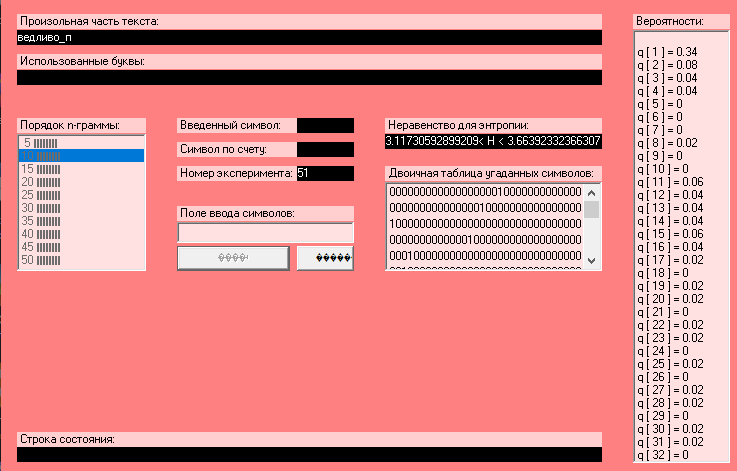
\includegraphics[width=.98\textwidth]{pics/pink1.png}

%\caption{}
\label{fig:overleaf}
\end{figure}

\begin{figure}[h!]
\centering
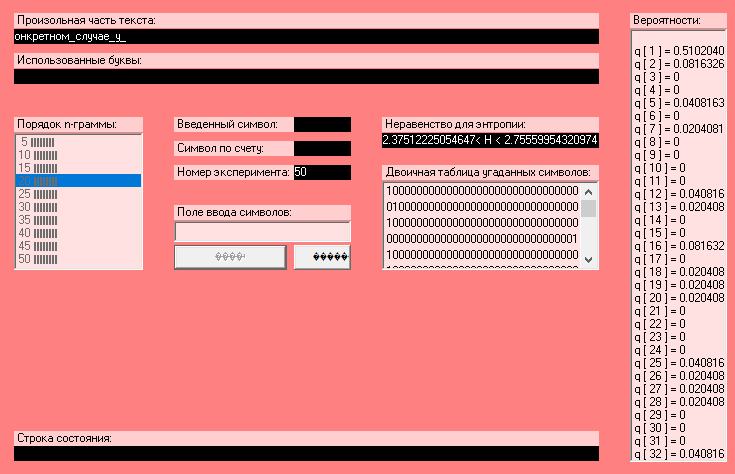
\includegraphics[width=.98\textwidth]{pics/pink2.png}

%\caption{}
\label{fig:overleaf}
\end{figure}

\begin{figure}[h!]
\centering
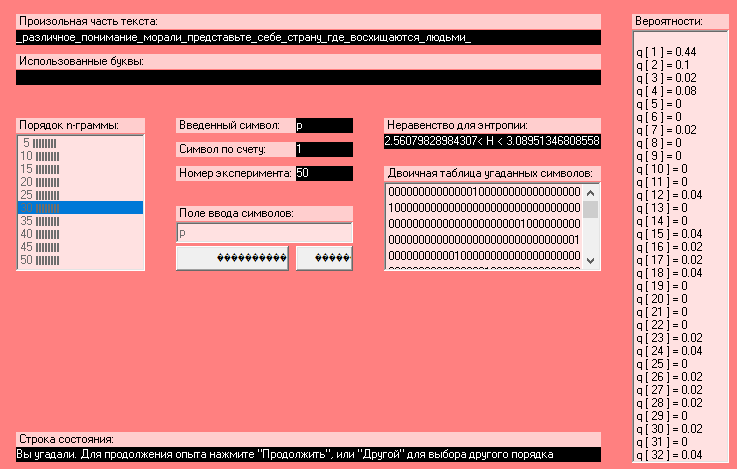
\includegraphics[width=.98\textwidth]{pics/pink3.png}

%\caption{}
\label{fig:overleaf}
\end{figure}


\section{Висновок}
Під час виконання даної лабораторної роботи я навчився вимірювати частоти символів та
біграм у тексті, визначати ентропію. Також, я навчився визначати надлишковість мови.